%\begin{enumerate}
%\item Clasificaci'on del juego:
\subsection{Clasificaci'on del juego}
\begin{itemize}
\item Este juego es sin azar.

\item Bipersonal, ya que intervienen dos jugadores, uno juega con las fichas blancas, el otro con las negras.

\item Es infinito, debido a que las jugadas posibles son infinitas. Esto se puede apreciar mejor en el grafo de estados del juego.

\item No es de Informaci'on Perfecta.

\item Es de Informaci'on Completa ya que tanto las estrategias como los pagos son conocidos por ambos jugadores al iniciar el juego.

\item No es un juego Cooperativo, como as'i tampoco de Movida Simult'anea, sino Secuencial.

\item Suma Cero. Ya que los pagos asociados son:
\begin{itemize}
\item 1, si el jugador gana.
\item -1, si el jugador pierde.
\item 0, si se llegara a empatar.
\end{itemize}
En un principio no hay empate pero, como es infinito porque se repiten jugadas, podr'ia forzarse con una regla del tipo \it{cuando se repita una cierta cantidad de veces una jugada se puede pedir el empate}.
\end{itemize}

%\item Grafo con todos los estados del juego:
\subsection{Grafo con todos los estados del juego}

Vamos a analizar tres juegos: 

\begin{itemize}
\item \it{Pong hau k'\ i}
\item \it{Pong hau k'\ i con una repetici'on}. Este es equivalente al anterior salvo porque al pasar por primera vez por un estado repetido se da fin al juego. El valor para este estado ser'a cero.
\item \it{Pong hau k'\ i sin repetici'on}. Tambi'en equivalente al primero. Pero ac'a la modificaci'on est'a en que no se puede tomar un camino que lleve a un nodo repetido. Se ver'a mejor en el gr'afico que viene a continuaci'on.
\end{itemize}


        \begin{figure}[p!hbt]
		\centering
		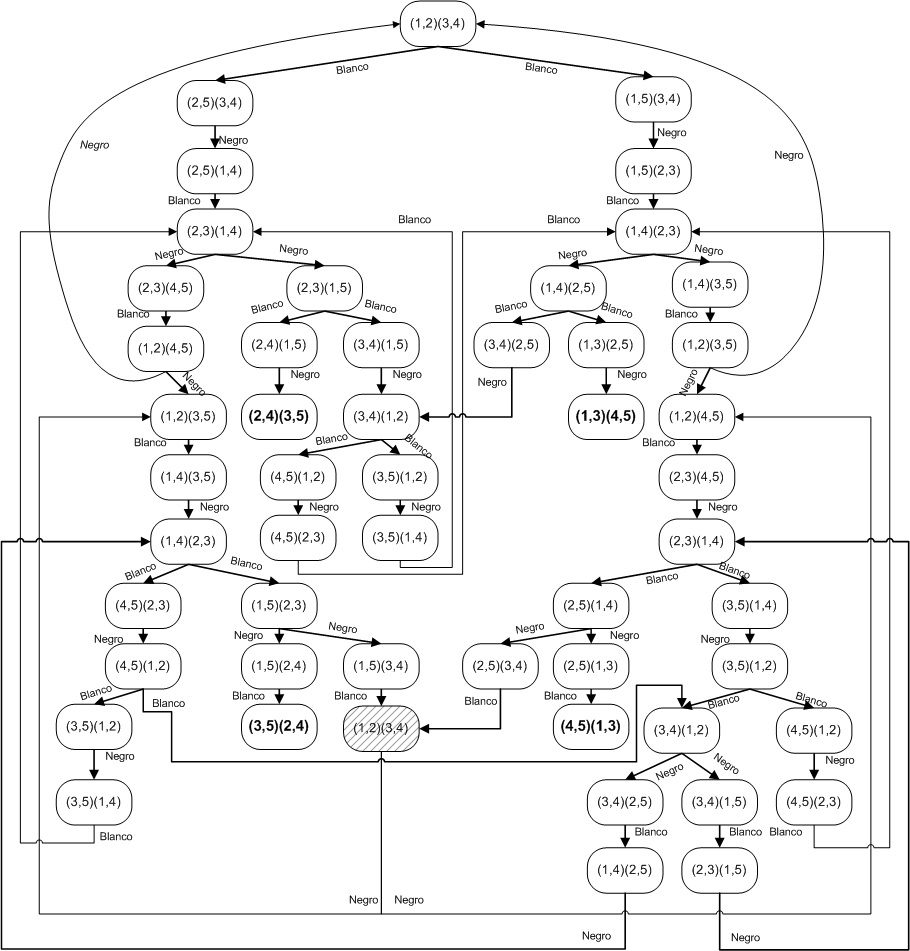
\includegraphics[angle=0, width=0.8\textwidth]{../img/GrafoPongInfinito.png}
		\caption{Juego Inifinito}
		\label{fig:Juego_Infinito}
	\end{figure}


%\item Valor del juego. Mejores estrategias.
%En un principio parece dificil determinarse a ciencia cierta si el juego tiene valor y m'as a'un, cu'al es dicho valor.

%Analisando el juego vimos que el \it{Pong hau k'\ i} es:

%\begin{itemize}
%\item de dos jugadores
%\item de informaci'on perfecta
%\end{itemize}

%Luego, aplicando el teorema de Kuhn, podemos asegurar que el juego \negrita{tiene valor}.



%Luego, si aplicamos la regla:
%$$cuando\ se\ repita\ una\ cierta\ cantidad\ de\ veces\ una\ jugada\ se\ puede\ pedir\ el\ empate$$
%Estar'iamos forzando a que sea finito, ya que no se podr'ian repetir las jugadas por siempre. Ahora tenemos un nuevo juego, llamemoslo \it{Pong hau k'\ i finito}

%Notar que el juego \it{Pong hau k'\ i} se reduce en \it{Pong hau k'\ i finito}, por lo tanto sus valores son iguales.


%\end{enumerate}
